\cleardoublepage
\appendix
\chapter{Complementary Definitions}\label{sec:complementsOfAlgebra}

\paragraph{Cartesian Space:} 3D Cartesian space defined by an X, Y, and Z axes (describing position based on horizontal placement, vertical placement, and depth respectively). The coordinates for any point within this space are shown as a vector $[x,y,z]$. The \emph{coordinate system} used this work is the right-handed system (thumbs points at the positive direction of x-axis, the index finger is pointing to the positive direction of y-axis, the positive  of z-axis given by remaining fingers).

\paragraph{Base Works:}\emph{Euler} outlined \emph{universal rotation theorem} which was presented in \cite{euler1775formulae}. Rigid body dynamics and rotation matrices defined by Schaub \cite{schaub2003analytical}. 

\paragraph{UAS Coordinate System:} \emph{Local Coordinate frame} is defined by UAS mass center as space center, $Z-$ in the direction of gravitational force, $X+$ in the direction of UAS heading. This local coordinate system is called Euler Normalized Unit-frame (ENU). 

\paragraph{Rotation Matrices:} Following \emph{Rotation Matrices} are used to transform between two displaced coordinate systems. Roll angle rotation is defined around X-axis by matrix (eq. \ref{eq:rollTransformationMatrix}) on YZ-plane. Pitch angle  rotation matrix is defined around Y-axis by matrix (eq. \ref{eq:pitchTransformationMatrix}) on XZ-plane. Yaw angle rotation matrix is defined around Z axis by matrix (eq. \ref{eq:yawTranformationMatrix}) on XY-plane.

\begin{equation}\label{eq:rollTransformationMatrix}
    R_{YZ} = R_{roll} =
    \begin{bmatrix}
        1 & 0 & 0\\
        0 & \cos(roll) & -\sin(roll)\\
        0 & \sin(roll) & \cos(roll)
    \end{bmatrix}
\end{equation}
\begin{equation}\label{eq:pitchTransformationMatrix}
    R_{XZ} = R_{pitch} =
    \begin{bmatrix}
        \cos(pitch) & 0 & \sin(pitch)\\
        0 & 1 & 0\\
        -\sin(pitch) & 0 & \cos(pitch)
    \end{bmatrix}
\end{equation}
\begin{equation}\label{eq:yawTranformationMatrix}
    R_{XY} = R_{yaw} = 
    \begin{bmatrix}
        \cos(yaw) & -\sin(yaw) & 0 \\
        \sin(yaw) & \cos(yaw) & 1 \\
        0 & 0 & 1
    \end{bmatrix}
\end{equation}
The full rotation matrix in X, Y, Z  is given by (eq. \ref{eq:xyzspaceRotationMatrix}).

\begin{equation}\label{eq:xyzspaceRotationMatrix}  
        R_{XYZ}  = R_{roll,pitch,yaw} =  R_{XY} * R_{XZ} * R_{YZ} = R_{yaw} * R_{pitch} *R_{roll}
\end{equation}

\begin{note}
    The rotation matrix $R_{XYZ}$ (eq. \ref{eq:xyzspaceRotationMatrix}) and its inverse $R_{XYZ}^{-1}$ which gives identity $R_{XYZ} \times R_{XYZ}^{-1} = I$ are used all over this work in transformation.
\end{note}

\paragraph{Gimbal Lock Prevention:} To keep solution numerically stable and rotations numerically stable gimbal lock prevention is necessary \cite{kramer1977gyro}. Gimbal lock occurs when one of the matrices (eq. \ref{eq:rollTransformationMatrix}, \ref{eq:pitchTransformationMatrix}, \ref{eq:yawTranformationMatrix}) is singular or final matrix for X, Y, Z rotation is singular (eq. \ref{eq:xyzspaceRotationMatrix}). Gimbal lock leads to the lost of one or more degree of freedom, depending on rank and space dimension of a singular matrix. To prevent gimbal lock, it is necessary to introduce a mechanism to check if the rotation matrix is regular. For this purpose normative reset function is introduced:


\begin{equation}
    \left [ roll, pitch , yaw \right ]^T = f(t,roll^-,pitch^-,yaw^-), \quad \textnormal{norm}(R_{roll,pitch, yaw})=3
\end{equation}


\noindent Function resets yaw or roll angle to the initial position to keep a degree (rank) of the rotation matrix. The simpler but not fault-tolerant solution is to keep angles $roll,pitch,yaw \in \left (  -\pi,\pi\right ]$ range.


\paragraph{Polar coordinates:} A \emph{polar coordinate system} represents a point in the form of vector:
\begin{equation*}
    point_{polar}=[distance, horizontal Dislocation Angle, vertical Dislocation Angle]^T
\end{equation*}
which is ideal for representation of LiDAR scanned point because usually total point distance and a pair of dislocation angles are returned. Using most common LiDAR with horizontal rotation $horizontal^\circ$ and vertical mirror inclination $vertical^\circ$, one can define polar coordinate $point_{polar} = [distance_{x,y,z},horizontal^\circ,vertical^\circ]$ which is dual to Cartesian coordinate $point_{cartesian} = [x,y,z]$. If rotation angle  ranges are $horizontal^\circ,vertical^\circ\in(-\pi,\pi]$ transformation function is a bijection.

\paragraph{Polar $\to$ Cartesian:} Transformation from polar to Cartesian representation is defined by following series of functions (eq. \ref{eq:cpt01}, \ref{eq:cpt02}, \ref{eq:cpt03}, \ref{eq:cpt04}).

\begin{equation}\label{eq:cpt01}
    distance_{xy} = \cos(horizontal^\circ)\times distance_{xyz}
\end{equation}

\begin{equation}\label{eq:cpt02}
    z = \sin(hirizontal^\circ)\times distance_{xyz}
\end{equation}

\begin{equation}\label{eq:cpt03}
    y = \sin(horizontal^\circ)\times distance_{xy}
\end{equation}

\begin{equation}\label{eq:cpt04}
    x = \cos(vertical^\circ) \times distance_{xy}
\end{equation}


\newpage
\paragraph{Cartesian $\to$ Polar:} Transformation from Cartesian to polar representation is defined by following series of functions (eq \ref{eq:cpt05}, \ref{eq:cpt06}, \ref{eq:cpt07}, \ref{eq:cpt08}).

\begin{equation}\label{eq:cpt05}
    distance_{xyz} = \sqrt{x^2+y^2+z^2}    
\end{equation}

\begin{equation}\label{eq:cpt06}
    distance_{xy} = \sqrt{x^2+y^2}    
\end{equation}

\begin{equation}\label{eq:cpt07}
    horizontal^\circ = \arctan\left(\frac{y}{x}\right)
\end{equation}

\begin{equation}\label{eq:cpt08}
    vertical^\circ =  \arctan \left( \frac{z}{d_{xy}}\right)
\end{equation}

\begin{definition}{Global Coordinate System (GCS) $\mathscr{X}_\mathscr{G}$}\label{def:globalCoordinateSystem}
    takes as center $c_{\mathscr{G}0}$ well-known point (for example center of geo-reference model in GNSS systems) every reference distance, plane or angle is calculated taking this center to mind.
\end{definition}

\begin{definition}{Local Coordinate System (LCS) $\mathscr{X}_\mathscr{L}$}\label{def:localCoordinateSystem}
    takes as center $c_{\mathscr{L}0}$ frame of the vehicle and can be changing position and orientation in global coordinate frame $\mathscr{X}_\mathscr{G}$.
\end{definition}

\begin{definition}{Global position of polar obstacle $o_i\in\mathscr{O}_{3D}$.}\label{def:globalObstaclePosition3D}
    Let $o_i = [d_o, \theta_o, \varphi_o]^T$ be polar position of obstacle $o_i$ in local coordinate frame of vehicle with global Cartesian position $[x,_v,y_v,z_v]^T$ and normalized orientation angles $[roll_v,pitch_v,yaw_v]$.\\
    
    Then Cartesian position of obstacle $oi$, $[x_o,y_o,z_o]^T$  in the local coordinate frame is given by transformation functions $x_o$ (eq. \ref{eq:cpt04}), $y_o$ (eq. \ref{eq:cpt03}), $z_o$ (eq. \ref{eq:cpt02}).\\ 
    
    Global  position of polar obstacle $oi$, $[x_g,y_g,z_g]^T$ is given by the following equation:
    \begin{equation}
        \begin{bmatrix}
            x_g\\y_g\\z_g
        \end{bmatrix}
        =
        \left [
            R_{XYZ}(roll_v,pitch_v,yaw_v)
            \begin{bmatrix}
                x_o\\y_o\\z_o
            \end{bmatrix}
            +
            \begin{bmatrix}
                x_v\\y_v\\z_v
            \end{bmatrix}
        \right ]
    \end{equation}    
\end{definition}

\begin{definition}{Local position of global coordinate $[x_g,y_g,z_g]^T\in\R^3$.}\label{def:globalToLocal}
    Let there be a vehicle with global Cartesian position $[x,_v,y_v,z_v]^T$ and normalized orientation angles $[roll_v,$ $pitch_v,$ $yaw_v]$. in global coordinate frame $\mathscr{X}_\mathscr{X}$.\\
    
    Then local Cartesian coordinate position $[x_l,y_l,z_l]^T$ of point $[x_g,y_g,z_g]^T$ is given by the the following equation:
    \begin{equation}
        \begin{bmatrix}
            x_l\\y_l\\z_l
        \end{bmatrix}
        =
        \left [
            R_{XYZ}(-roll_v,-pitch_v,-yaw_v)
            \left (
            \begin{bmatrix}
                x_g\\y_g\\z_g
            \end{bmatrix}
            -
            \begin{bmatrix}
                x_v\\y_v\\z_v
            \end{bmatrix}
            \right )
        \right ]
    \end{equation}
    
    The local polar position is given as $[distance_l, horizontal_l^\circ,horizontal_l^\circ]$, where $distance_l$ is given by (eq. \ref{eq:cpt05}), $vertical_l^\circ$ is given by (eq. \ref{eq:cpt07}). $vertical_l^\circ$ is given by (eq. \ref{eq:cpt08}), where $[x_l,y_l,z_l]$ are used as local coordinates.
\end{definition}

\newpage
\paragraph{Polar surface calculation:} The problem is to calculate intersected surface $dA$ of ball subsurface defined by radius $r$, horizontal span $\phi$, and vertical span $\theta$. From classical mechanics, one can formulate the problem as given by (fig. \ref{fig:80BallSpan}). The intersection plot is in (fig. \ref{fig:81BallSpan2}).

\begin{figure}[H]
    \centering
    \begin{subfigure}[H]{0.3\textwidth}
        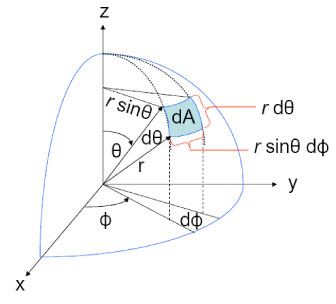
\includegraphics[width=\textwidth]{\FIGDIR/80BallSpan.jpg}
        \caption{Notation}
        \label{fig:80BallSpan}
    \end{subfigure}
    \begin{subfigure}[H]{0.3\textwidth}
        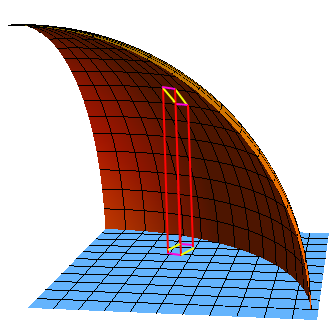
\includegraphics[width=\textwidth]{\FIGDIR/81BallSpan2.png}
        \caption{Plot}
        \label{fig:81BallSpan2}
    \end{subfigure}
    \caption{Polar surface calculation notation and plot}
    \label{fig:BallSpanNOTPLOT}
\end{figure}

\noindent One can use the first fundamental form to determine the surface area element. Recall that this is the metric tensor, whose components are obtained by taking the inner product of two tangent vectors in polar space $g_{i,j}= X_i \cdot X_j$, for tangent vectors $X_i$, $X_j$. Following identification for the components of metric tensor will be used:
\begin{equation}\label{eq:metricTensorIdentification}
    g_{ij}=
    \begin{bmatrix}
        E&F\\
        F&G
    \end{bmatrix}
\end{equation}

\noindent Where $E=<X_u,X_u>$, $F=<X_u,X_v>$, and $G=<X_v,X_v>$. Lagrange`s identity can be used, which tells us that the squared area of a parallelogram in space is equal to the sum of the squares of its projections onto the Cartesian plane:
\begin{equation}\label{eq:CartesianProjectionIdentity}
    |X_u \times X_v|^2 = |X_u|^2|X_v|^2 - \left(X_u\cdot X_v\right)^2
\end{equation}

\noindent Given example is displayed in (fig. \ref{fig:81BallSpan2}). The area element is given as:
\begin{equation}\label{eq:squareElementSurfaceDerivation}
    \begin{aligned}
    \text{d}A &= |X_u \times X_v| \quad\text{d}u\text{d}v \\
    & = \sqrt{\left||X_u|^2|X_v|^2 - \left(X_u\cdot X_v\right)^2\right|}\quad \text{d}u\text{d}v\\ 
    & = \sqrt{EG-F^2} \quad \text{d}u\text{d}v
    \end{aligned}
\end{equation}

\noindent We will find tangent vectors via the usual parametrization which give, $X(\phi,\theta)$ = $[r \cos\phi\sin\theta,$ $r\sin\phi\sin\theta,$ $r\cos\theta]$, so that tangent vectors are simply defined as:
\begin{equation}\label{eq:tangentVectorsForPlanarSurface}
    \begin{aligned}
        X_\phi &= [-r\sin\phi\cos\theta,r\cos\phi\sin\theta,0]\\
        X_\theta &=[-r\cos\phi\sin\theta,r\sin\phi\cos\theta,-r\sin\theta]
    \end{aligned}
\end{equation}

\noindent Computing the elements of the first fundamental form gives us:
\begin{equation}
    E = r^2\cos^2\theta,\quad F=0,\quad G=r^2
\end{equation}

\noindent Thus final difference is given as:
\begin{equation}\label{eq:finalCellSquareNice}
    \text{d}A=\sqrt{r^4\cos^2}\quad \text{d}\theta\text{d}\phi = r^2 \cos\theta\quad \text{d}\theta\text{d}\phi
\end{equation}

\begin{note} 
    \emph{Polar Surface} is used in \emph{Detected Obstacle Rating Calculation} (eq. \ref{eq:naiveObstacleRate}). The final formula used in the \emph{surface integral calculation} in \emph{non-compact notation} is given as the following:

    \begin{equation}\label{eq:finalCellSquare}
        \text{d}A= r^2 \cos(horizontal^\circ)\quad \text{d}horizontal^\circ \text{d}vertical^\circ
    \end{equation}
\end{note}